\section{Duas variáveis aleatórias}

Seja $(X, Y)$ um vetor aleatório.

\subsection{Vetor aleatório para variável aleatória}
Considere $Z = H(X, Y)$.

\begin{example}
    Algumas transformações $Z = H(X, Y)$:
    \begin{enumerate}[label=(\roman*)]
        \item $Z = XY$
        \item $Z = X + Y$
        \item $Z = \sqrt{X^2 + Y^2}$
    \end{enumerate}
\end{example}

Se $X$ e $Y$ forem \va s discretas, então $Z$ também
será discreta, com valores que dependem de $X$ e $Y$
e da transformação $H$.

Temos:
\begin{align}
    \Prob(Z = z) = \Prob(H(X, Y) = z)
    &= \underset{(x, y) : H(x, y) = z}{\sum\sum}
        \Prob(X = x, Y = y)
\end{align}

Se $X$ e $Y$ forem \va s contínuas e $H(x, y)$ for uma função
contínua, então $Z$ é uma \va\ contínua. Temos:
\begin{align}
    F_Z(z) = \Prob(Z \le z) = \Prob(H(X, Y) \le z)
    &= \iint_{B(z)} f_{X,Y}(x, y) \wrt x \wrt y
\end{align}
sendo que
\begin{align*}
    B(z) &= \{(x, y) : H(x, y) \le z \}.
\end{align*}

Derivando $F_Z(z)$, obtemos:
\begin{align*}
    f_Z(z) &= \diff{}{z} F_Z(z)
\end{align*}

\subsection{Vetor aleatório para vetor aleatório}
Considere, agora, $Z = H_1(X, Y)$ e $W = H_2(X, Y)$.
Deseja-se determinar a distribuição de $(Z, W)$.

Se $X$ e $Y$ são \va s discretas, então $Z$ e $W$
também são. Neste caso:
\begin{align*}
    \Prob(Z = z, W = w) &= \Prob(H_1(X, Y) = z, H_2(X, Y) = w) \\
    &= \underset{\substack{(x,y) : H_1(x, y) = z,\\
        H_2(x, y) = w}} {\sum\sum} \Prob(X = x, Y = y)
\end{align*}

Considere agora $(X, Y)$ um vetor contínuo.

\begin{theorem}\label{def:ch04-metodo-jac-vetor}
    Suponha que as equações $z = H_1(x, y)$ e $w = H_2(x, y)$
    tenham solução única $x = G_1(z, w)$ e $y = G_2(z, w)$. Além
    disso, suponha que as derivadas parciais $\diffp{G_1}{z}$,
    $\diffp{G_1}{w}$, $\diffp{G_2}{z}$ e $\diffp{G_2}{w}$
    são contínuas. Então, a função densidade do vetor $(Z, W)$
    é dada por:
    \begin{align}
        f_{Z,W}(z, w) &= f_{X, Y}(G_1(z, w), G_2(z, w))
            \cdot |\det\ J|
        \label{eq:ch04-metodo-jac-vetor}
    \end{align}
    sendo que $J$ é a matriz jacobiana, dada por:
    \begin{align*}
        J &= \begin{bmatrix}
            \diffp{G_1}{z} & \diffp{G_1}{w} \\[10pt]
            \diffp{G_2}{z} & \diffp{G_2}{w} \\
        \end{bmatrix}
    \end{align*}
\end{theorem}

\begin{notation}
    Algumas referências utilizam a seguinte noteção
    para a matriz jacobiana:
    \begin{align*}
        J &= \diffp{{(G_1, G_2)}}{{(z, w)}}
    \end{align*}
\end{notation}

Em alguns problemas, o objetivo é obter a função densidade
de $Z$ (que é a densidade marginal em $Z$ do vetor $(Z, W)$).
Para tal, calculamos:
\begin{align*}
    f_Z(z) &= \int_{-\infty}^{+\infty} f_{Z, W}(z, w) \wrt w
\end{align*}
Neste caso, a variável $W$ representa uma transformação
auxiliar que é escolhida para facilitar os cálculos.
Por exemplo, podemos escolher $W = H_2(X, Y) = X$ ou
$W = H_2(X, Y) = Y$.

\begin{example}
    Tiro ao alvo em um alvo circular de forma aleatória.
    O raio do círculo é igual a 1. A posição do tiro
    tem coordenadas $(X, Y)$. O vetor $(X, Y)$ tem função
    densidade
    \begin{align*}
        f_{X,Y}(x,y) &= \begin{cases}
            \frac{1}{\pi} &,\ \text{se } 0 < x^2 + y^2 \le 1 
                \\[10pt]
            0 &,\ \text{caso contrário.}
        \end{cases}
    \end{align*}
    Considere
    \begin{align*}
        Z = H_1(X, Y) &= \sqrt{X^2 + Y^2} \in (0, 1).
    \end{align*}
    Obter a função densidade de $Z$.

    \bigskip
    Definimos a variável auxiliar 
    $W = \arctan\left(\frac{Y}{X}\right)$.
    
    \begin{center}
        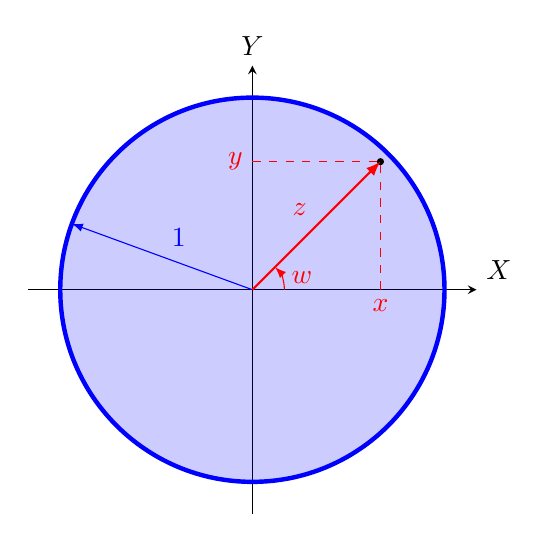
\begin{tikzpicture}[
                declare function={
                    F(\x) = sqrt(\x/pi);
                }
            ]
            \begin{axis}[
                unbounded coords=jump,
                grid=none,
                axis x line=middle,
                axis y line=middle,
                xmin=-3.5, xmax=3.5,
                ymin=-3.5, ymax=3.5,
                xtick=\empty,
                ytick=\empty,
                xlabel={$X$},
                ylabel={$Y$},
                x label style={anchor=south west},
                y label style={anchor=south},
                legend style={fill=none,draw=none},
                unit vector ratio={1 1},
            ]

            \coordinate (O) at (0,0);
            \coordinate (P) at (2, 2);
            \coordinate (Px) at (2, 0);
            \coordinate (Py) at (0, 2);

            \draw[fill, blue, ultra thick, fill opacity=0.2]
                (O) circle (3);

            \draw[fill] (P) circle (.25ex);

            \draw[-latex, blue] (O) -- (-2.82, 1.03);
            \node[blue, anchor=south west] at (-1.41, 0.52) {$1$};
            
            \draw[-latex, red, thick] (O) -- (P);
            \draw[red, dashed, thin] (Px) -- (P);
            \draw[red, dashed, thin] (Py) -- (P);
            
            \draw[-latex, red] (0.5, 0) arc (0:45:0.5);

            \node[anchor=north, red] at (Px) {$x$};
            \node[anchor=east, red] at (Py) {$y$};
            \node[anchor=south east, red] at (1, 1) {$z$};
            \node[anchor=west, red] at (0.46, 0.19) {$w$};

            \end{axis}
        \end{tikzpicture}
    \end{center}

    Resolvendo as duas equações
    \begin{align*}
        z = H_1(x, y) &= \sqrt{x^2 + y^2} \\
        w = H_2(x, y) &= \arctan\left(\frac{Y}{X}\right)
    \end{align*}
    obtemos
    \begin{align*}
        x = G_1(z, w) &= z \cdot \cos\ w \\
        y = G_2(z, w) &= z \cdot \sen\ w \\
    \end{align*}

    Calculamos
    \begin{align*}
        J &= \begin{bmatrix}
            \diffp{G_1}{z} & \diffp{G_1}{w} \\[10pt]
            \diffp{G_2}{z} & \diffp{G_2}{w} \\
        \end{bmatrix}
        = \begin{bmatrix}
            \cos\ w & -z\cdot\sen\ w \\
            \sen\ w & z\cdot\cos\ w \\
        \end{bmatrix}
    \end{align*}
    de modo que
    \begin{align*}
        \det\ J &= \begin{vmatrix}
            \cos\ w & -z\cdot\sen\ w \\
            \sen\ w & z\cdot\cos\ w \\
        \end{vmatrix} \\
        &= \cos\ w \cdot z\cdot\cos\ w
        - (-z\cdot\sen\ w) \cdot \sen\ w \\
        &= z\cdot \cos^2 w + z\cdot \sen^2 w \\
        &= z\cdot (\cos^2 w + \sen^2 w) = z
    \end{align*}

    Logo:
    \begin{align*}
        f_{Z,W}(z, w) &= f_{X, Y}(G_1(z, w), G_2(z, w))
            \cdot |\det\ J| \\
        &= \frac{1}{\pi} \cdot |z| = \frac{z}{\pi}
    \end{align*}
    se $0 < z < 1$ e $0 < w < 2\pi$.

    Portanto, a função densidade de $Z$ é:
    \begin{align*}
        f_Z(z) &= \int_0^{2\pi} f_{Z, W}(z,w) \wrt w \\
        &= \int_0^{2\pi} \frac{z}{\pi} \wrt w
        = \frac{z}{\pi} \int_0^{2\pi} \wrt w
        = \frac{z}{\pi} \cdot 2\pi = 2z
    \end{align*}
    para $0 < z < 1$.

    \begin{center}
        \begin{tikzpicture}
            \begin{axis}[
                unbounded coords=jump,
                grid=major,
                axis x line=middle,
                axis y line=middle,
                xmin=-1, xmax=2,
                ymin=0, ymax=2.2,
                xtick={1},
                ytick={2},
                xlabel={$z$},
                ylabel={$f_Z(z)$},
                x label style={anchor=south west},
                y label style={anchor=south},
                legend style={fill=none,draw=none},
            ]

            \addplot[ultra thick, blue, samples at={0,1}]
                {2*x};
            \addplot[ultra thick, blue, samples at={-1, 0}]
                {0};
            \addplot[ultra thick, blue, samples at={1, 2}]
                {0};
            \addplot[ultra thick, blue, only marks, fill=white]
                coordinates {(1, 2)};
            \addplot[ultra thick, blue, only marks]
                coordinates {(0, 0) (1, 0)};

            \end{axis}
        \end{tikzpicture}
    \end{center}

    \bigskip
    \textbf{Outro método}

    Temos
    \begin{align*}
        F_Z(z) = \Prob(Z \le z)
        &= \Prob(\sqrt{X^2 + Y^2} \le z) \\
        &= \Prob(X^2 + Y^2 \le z^2) \\
        &= \Prob((X, Y) \in B(z))
    \end{align*}
    sendo que
    \begin{align*}
        B(z) &= \{(x, y) \in \R^2 : x^2 + y^2 \le z^2\}
    \end{align*}
    para $0 < z < 1$. Calculamos:
    \begin{align*}
        F_Z(z) &= \Prob((X, Y) \in B(z)) \\
        &= \iint_{B(z)} f_{X, Y}(x, y) \wrt x \wrt y \\
        &= \iint_{B(z)} \frac{1}{\pi} \wrt x \wrt y \\
        &= \frac{1}{\pi} \iint_{B(z)} \wrt x \wrt y \\
        &= \frac{1}{\pi} \cdot \area(B(z)) \\
        &= \frac{1}{\pi} \cdot \pi z^2  = z^2\\
    \end{align*}

    Portanto, a função densidade é dada por
    \begin{align*}
        f_Z(z) &= \diff{}{z}F_Z(z) = 2z,\ 0 < z < 1.
    \end{align*}
\end{example}
